% Teilaufgabe X

\section{Signal vor dem Mischer bei fester Modulationsfrequenz $\omega_\mathrm{m}$}
\label{sec:signalMischer}

Wenn phasenmoduliertes  Licht  auf  einen  Photodetektor fällt, erzeugt jede der Seitenbanden mit der Trägerlinie eine Schwebung der Frequenz $\omega_\mathrm{m}$. Die beiden Schwebungen haben gleiche Amplituden und sind um $\pi$ phasenverschoben und löschen sich aus. Der Photodetektor liefert nur ein Gleichstromsignal, aber kein Signal bei der Modulationsfrequenz $\omega_\mathrm{m}$. 

Wenn auf dem Weg zwischen Modulator und Detektor eine Probe mit einer schmalen Absorptionslinie im Strahlengang steht, kann z. B. die positive Seitenbande durch die Absorptionslinie abgeschwächt wird und die negative nicht. Überwiegt die negative Schwebung gegen über der positiven, registriert der Detektor ein Wechselstromsignal der Kreisfrequenz $\omega_\mathrm{m}$. Insgesamt registriert der Photodetektor im Grenzfall schwacher Absorptionslinien also folgendes Lichtsignal:
\begin{gather}
    \begin{aligned}
        I(t) &= I_0 e^{-2\delta_0}\left[ 1 + (\delta_{-1} - \delta_{1})M\cos(\omega_\mathrm{m}t) + (\phi_{-1} + \phi_{1} - 2\phi_0)M\sin(\omega_\mathrm{m}t) \right]\\
             &= \text{Abschw\"achung}\left[1 + \mathrm{Absorption} + \mathrm{Dispersion}\right]~,
    \end{aligned}
    \label{eq:signal}
\end{gather}
wobei $\delta_\mathrm{n}$ sind die Amplituden-Absorptionskoeffizienten der Probe für die Seitenbande und die Trägerlinie und $\phi_\mathrm{n}$ die Phasenverschiebungen, die die drei Linien beim Durchgang durch die Probe erfahren. Ohne Probe arbeitet die Methode hintergrundfrei. Gleichung (\ref{eq:signal}) beschreibt dann Skizze in Abbildung \ref{fig:signal}. \cite{anleitung}
\begin{center}
    \captionsetup{type=figure}
    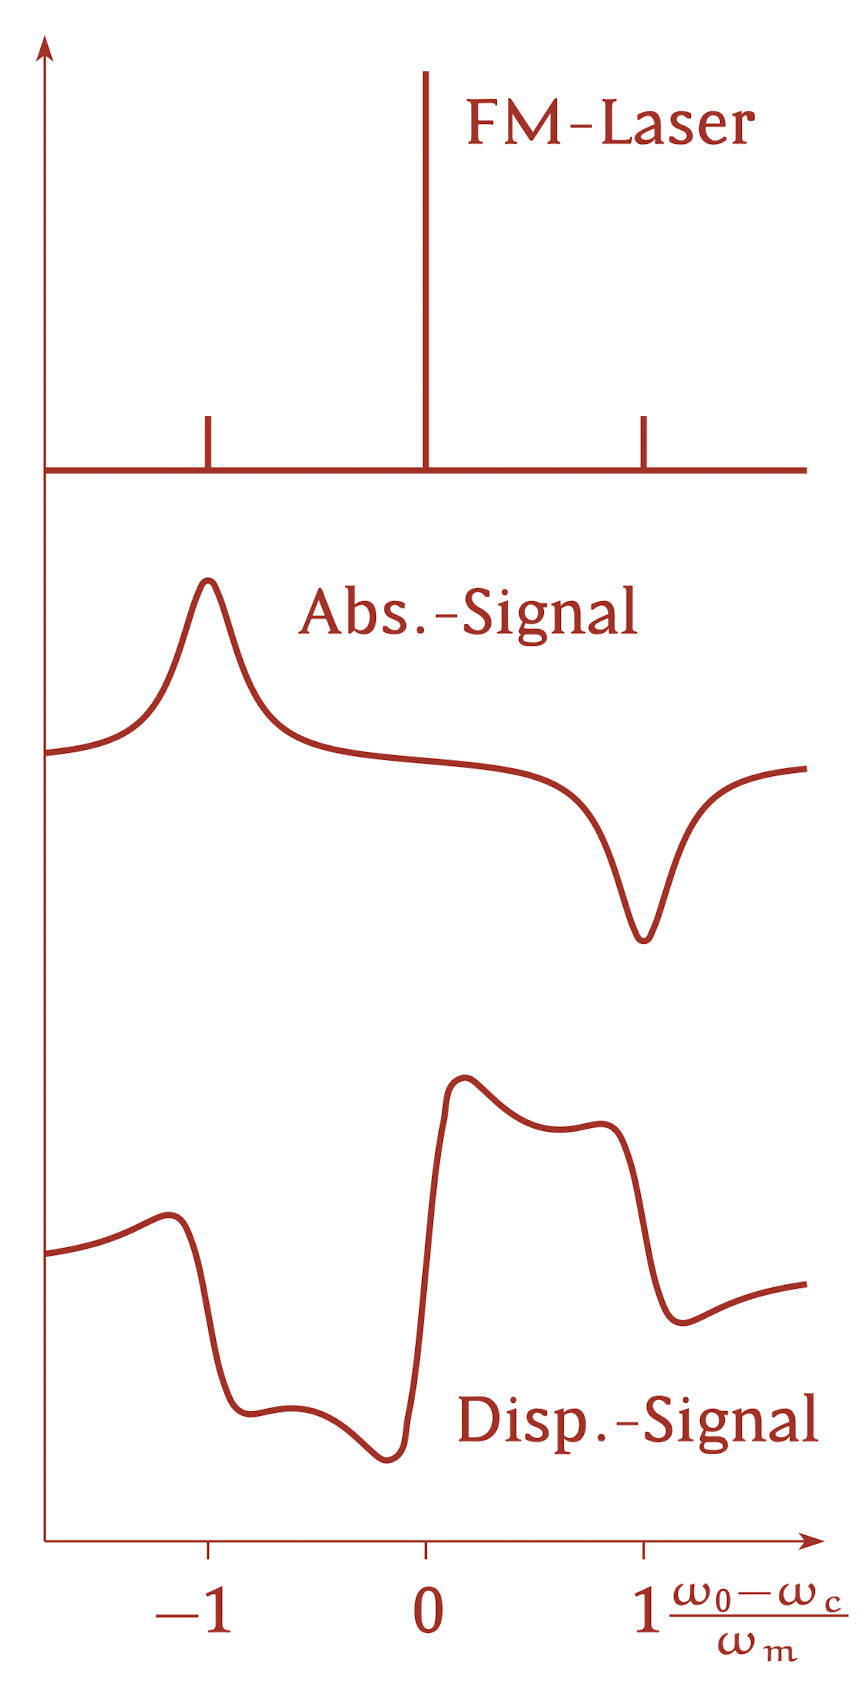
\includegraphics[width=0.3\textwidth]{Bilder/Signal.png}
    \captionof{figure}{Signal im Photodetektor mit Probe im Strahlengang bei schwacher Absorptionslinien \cite{anleitung}}
    \label{fig:signal}
\end{center}